\documentclass[9pt, aspectratio=169]{beamer}

\usetheme{metropolis}
\setbeamertemplate{itemize items}{\faAngleRight}

\metroset{titleformat=smallcaps,block=fill,numbering=counter,progressbar=frametitle,sectionpage=none}
\setbeamersize{text margin left=5mm,text margin right=5mm} 
% \input{embed_video}
\usepackage{fontspec,minted}
\usepackage[scale=1]{ccicons}
\usepackage{metalogo}
\usepackage{xcolor,colortbl}
\usepackage{multicol,multirow,booktabs}
\usepackage{appendixnumberbeamer}
\usepackage{graphicx}
\usepackage{mismath}
\usepackage{bm}
\usepackage{fontawesome5}
\usepackage{csquotes}
\usepackage[backend=biber, natbib, sorting=nyt, doi=true, url=false, url=false, isbn=false, maxbibnames=10]{biblatex}
\addbibresource{../utils/refs.bib}

\usepackage[spanish, es-nodecimaldot]{babel}
\deftranslation[to=spanish]{Definition}{Definición}
\deftranslation[to=spanish]{Theorem}{Teorema}
\deftranslation[to=spanish]{Example}{Ejemplo}

\usepackage{mathtools, mathrsfs}
\usefonttheme{professionalfonts}
\usepackage{textcomp, wasysym}

\setsansfont[BoldFont={Iwona Heavy}, Numbers={Lining, Proportional}]{Iwona Light}
\setmonofont[Scale=MatchLowercase]{Hack Nerd Font Mono}

\setbeamercolor{alerted text}{fg=red,bg=black!2}
\setbeamercolor{progress bar}{fg=red,bg=red!2}
\setbeamertemplate{itemize item}{\faCaretRight}
\setbeamertemplate{itemize subitem}{ \faAngleRight}
\setbeamertemplate{blocks}[shadow=false]
\setbeamercolor{block title}{bg=black!30,fg=red}
\setbeamercolor{block body}{bg=black!20,fg=black}
\setbeamertemplate{theorem begin}
{%
\begin{\inserttheoremblockenv}
{%
\inserttheoremheadfont
%{Teorema:}
\inserttheoremname
\ifx\inserttheoremaddition\@empty\else\ : \inserttheoremaddition\fi%
\inserttheorempunctuation
}%
}
\setbeamertemplate{theorem end}{\end{\inserttheoremblockenv}}
\makeatother


 
\usepackage{gensymb,amssymb}
\usepackage{siunitx}
\DeclareSIUnit{\nada}{\relax}
\usepackage{upquote}
\usepackage{cancel}
\usepackage{algpseudocode}
\algrenewcommand\algorithmicrequire{\textbf{Requiere}}
\algrenewcommand\algorithmicensure{\textbf{Devuelve}}
\setbeamertemplate{blocks}[shadow=false]

\newcommand{\cx}{\column{0.5\textwidth}}
\newcommand{\cw}[1]{\column{#1\textwidth}}

\author{Manuel Carlevaro}
\date{{\tiny Departamento de Ingeniería Mecánica \\
             Grupo de Materiales Granulares - UTN FRLP \\
             manuel.carlevaro@gmail.com }}
\institute{
  \vspace{6em}
  \centering
  {\tiny
  Cálculo Avanzado \enspace • \enspace 2025 \\
    \faLinux \- $\cdot$ \- \fontspec{TeX Gyre Pagella}\XeLaTeX \- $\cdot$ \- \ccbysa }
}

%% Operadores
\DeclareMathOperator{\sen}{sen}
\DeclareMathOperator{\senc}{senc}
\DeclareMathOperator{\sign}{sign}
\DeclareMathOperator{\Tr}{Tr}
\DeclareMathOperator{\rg}{rg}
\DeclareMathOperator{\cond}{cond}
\newcommand{\T}[1]{\underline{\bm{#1}}}
\newcommand{\uvec}[1]{\hat{\bm{#1}}}

\usepackage{hyperref}
\hypersetup{
    colorlinks,
    citecolor=blue,
    filecolor=black,
    linkcolor=blue,
    urlcolor=blue
}
\urlstyle{same}

%% Códigos
\usepackage{minted}
\newminted[cpp]{cpp}{linenos,fontsize=\footnotesize,frame=lines,numbersep=4pt}
\newmintedfile[cppcode]{cpp}{linenos,fontsize=\footnotesize,frame=lines,numbersep=4pt}
\newcommand{\mic}[1]{\mintinline{C++}{#1}}

\newminted[py]{python}{linenos,fontsize=\footnotesize,frame=lines,numbersep=4pt}
\newminted[pyc]{pycon}{linenos,fontsize=\footnotesize,frame=lines,numbersep=4pt} % Consola de Python
\newminted[ipy3]{ipython3}{linenos,fontsize=\footnotesize,frame=lines,numbersep=4pt} % Consola de iPython3
\newmintedfile[pycode]{python}{linenos,fontsize=\footnotesize,frame=lines,numbersep=4pt}

\newmintedfile[makef]{basemake}{linenos,fontsize=\footnotesize,frame=lines,numbersep=4pt}
\definecolor{bg}{RGB}{22,43,58}
\newminted[shell]{console}{linenos=false,fontsize=\footnotesize,breaklines=true, frame=single} % Linea de comandos
\renewcommand\listingscaption{Código}

\makeatletter
\AtBeginEnvironment{minted}{\dontdofcolorbox}
\def\dontdofcolorbox{\renewcommand\fcolorbox[4][]{##4}}
\makeatother

% uso:
% Ejemplo de uso explícito:
% \begin{py}
% >>> list("abcd")
% ['a', 'b', 'c', 'd']
% \end{py}
% 
% Ahora ejemplo de código en file:
% \pycode{Chapters/intro/code/hola.py}
% 
% También se puede poner un sector del file:
% \pycode[firstline=6, lastline=7]{Chapters/intro/code/hola.py}
% 
% También se puede poner código \textit{inline}: \mip{print('¡Hola mundo!')} y en una sola línea:
% \slp|if __name__ == '__main__')|
% 
% Por último, se puede poner el código en un entorno \textit{float}, esto es, como las tablas y las figuras, con un caption y un label para luego hacer referencias, como por ejemplo al Código \ref{code:hola}.


\usepackage{tikz}
\usetikzlibrary{shapes,shadows,arrows,positioning,matrix,chains,backgrounds,fit}

\tikzset{
    %Define standard arrow tip
    >=stealth',
    %Define style for boxes
    obj/.style={
           rectangle,
           rounded corners,
           draw, very thick,
           text width=10em, fill=green!20,
           minimum height=2em,
           text centered, drop shadow},
    proc/.style={
	    rectangle, rounded corners,
	    draw,fill=red!50,very thick,
	    text width=8em,minimum height=2em,
	    text centered, drop shadow},
    % Define arrow style
    pil/.style={
           ->,
           thick,
           shorten <=2pt,
           shorten >=2pt,}
}

\setbeamertemplate{bibliography item}{%
  \ifboolexpr{ test {\ifentrytype{book}} or test {\ifentrytype{mvbook}}
    or test {\ifentrytype{collection}} or test {\ifentrytype{mvcollection}}
    or test {\ifentrytype{reference}} or test {\ifentrytype{mvreference}} }
    {\setbeamertemplate{bibliography item}{\faBook}}
    {\ifentrytype{online}
            {\setbeamertemplate{bibliography item}{\faGlobe}}
   {\setbeamertemplate{bibliography item}{\faFileText}}}%
  \usebeamertemplate{bibliography item}}

\defbibenvironment{bibliography}
  {\list{}
     {\settowidth{\labelwidth}{\usebeamertemplate{bibliography item}}%
      \setlength{\leftmargin}{\labelwidth}%
      \setlength{\labelsep}{\biblabelsep}%
      \addtolength{\leftmargin}{\labelsep}%
      \setlength{\itemsep}{\bibitemsep}%
      \setlength{\parsep}{\bibparsep}}}
  {\endlist}
  {\item}
\newcommand{\bcite}[1]{\citeauthor{#1}, \citetitle{#1} (\citeyear{#1})}


\title{Serie y Transformada de Fourier}
\subtitle{Funciones ortogonales. Series de Fourier. Integral de Fourier. Transformada seno y coseno. Transformada de Fourier. Ejemplos.}

%%
%% ver: https://youtu.be/ZYf0tz9oVz8?si=njTb4eYMM7jol9Ru
%%



\begin{document}
\maketitle

\begin{frame}{ Funciones ortogonales }
\begin{columns}[t]
\cw{0.3}
Secuencia infinita $\{\phi_n(x)\}$ integrable en $[a, b]$ y
\[ \int_a^b \phi_i(x) \phi_j(x) \, dx = 0, \quad i \neq j \]
\pause

\vspace{-1em}
familia \alert{ortogonal} de funciones en $[a, b]$. Supongamos que existe
\[ \int_a^b f(x) \, dx \]
y
\[ f(x) = \sum_{n = 1}^{\infty} c_n \phi_n(x) \]
\[c_3 = \color{red}{?} \]
\[ f(x) \phi_3(x) = \sum_{i = 1}^{\infty} c_n \phi_n(x) \phi_3(x) \]
\pause

\cw{0.3} \vspace{-1.5em}
\begin{multline*}
\int_a^b f(x) \phi_3(x) \, dx = \\
\int_a^b \sum_{i = 1}^{\infty} c_n \phi_n(x) \phi_3(x) \, dx = \\
\sum_{i = 1}^{\infty} \int_a^b c_n \phi_n(x) \phi_3(x) \, dx = \\
c_3 \int_a^b \phi_3^2(x) \, dx
\end{multline*}
\begin{equation}
c_k = \frac{\int_a^b f(x) \phi_k(x) \, dx}{\int_a^b \phi_k^2(x) \, dx} 
\label{eq:ck}
\end{equation}
\pause

\begin{definition}
Producto interno:
\[ \langle f, g \rangle = \int_a^b f(x) \, g(x) \, dx \]
\end{definition}
\cw{0.3}
Con $c_k$ definida por \eqref{eq:ck}:
\[f(x) \sim \sum_{n = 1}^{\infty} c_n \phi_n(x) = F(x) \]
$F(x)$ es la \textbf{representación de Fourier} de $f(x)$ con respecto de $\{\phi_n(x)\}$.

Se puede demostrar:
\begin{multline*}
    \int_a^{b} \left[ f(x) - \sum_{k = 1}^n c_k \phi_k(x) \right]^2 \, dx \leq \\
    \int_a^{b} \left[ f(x) - \sum_{k = 1}^n d_k \phi_k(x) \right]^2 \, dx 
\end{multline*}
\end{columns}
\end{frame}

\begin{frame}
\begin{columns}[t]
\cx
\textbf{Caso especial:}
\begin{multline*}
\{1, \cos x, \cos 2x, \cos 3x, \cdots, \\
\sen x, \sen 2x, \sen 3x,  \cdots \} 
\end{multline*}
$\mapsto$ conjunto ortogonal en $[-\pi, \pi]$.

Por ejemplo, si $m \neq n$:
\begin{multline*}
\int_{-\pi}^{\pi} \cos mx \, \cos nx \, dx = \\
\frac{1}{2} \int_{-\pi}^{\pi} [\cos(m + n) x + \cos(m - n) x] \, dx = \\
\frac{1}{2} \left[ \frac{\sen(m + n) x}{m + n} + \frac{\sen(m-n) x}{m - n} \right]_{x = -\pi}^{\pi} \\
= 0
\end{multline*}
\pause

\cx
\textbf{Resultado clave:}

Supongamos que $f(x)$ sea suave a tramos en $[-\pi, \pi]$, y que
\[ F(x) = \sum_{n = 0}^{\infty} a_n \cos nx + \sum_{n = 0}^{\infty} b_n \sen nx \]
es la representación de Fourier de $f(x)$. Entonces, para $x_0 \in [-\pi, \pi]$:
\[ F(x_0) = \frac{f(x_0^+) + f(x_0^-)}{2} \]

\begin{exampleblock}{Ejemplo:}
    \begin{equation*}
        f(x) = \begin{cases}
            -1, &-\pi \leq x < 0 \\
            \phantom{-}1, &0 \leq x < \pi
        \end{cases}
    \end{equation*}
\end{exampleblock}
\end{columns}
\end{frame}

\begin{frame}
\begin{columns}[t]
\cx
\begin{align*}
F(x) &= \frac{4}{\pi} \sum_{n \text{ impar}}^{\infty} \frac{\sen nx}{n} =  \frac{4}{\pi} \sum_{n = 0}^{\infty} \frac{\sen (2 n + 1) x}{2 n + 1}\\
     &= \frac{4}{\pi} \left( \sen x + \frac{\sen 3x}{3} + \frac{\sen 5 x}{5} + \cdots \right)
\end{align*}
Primeros dos términos:
\begin{center}
    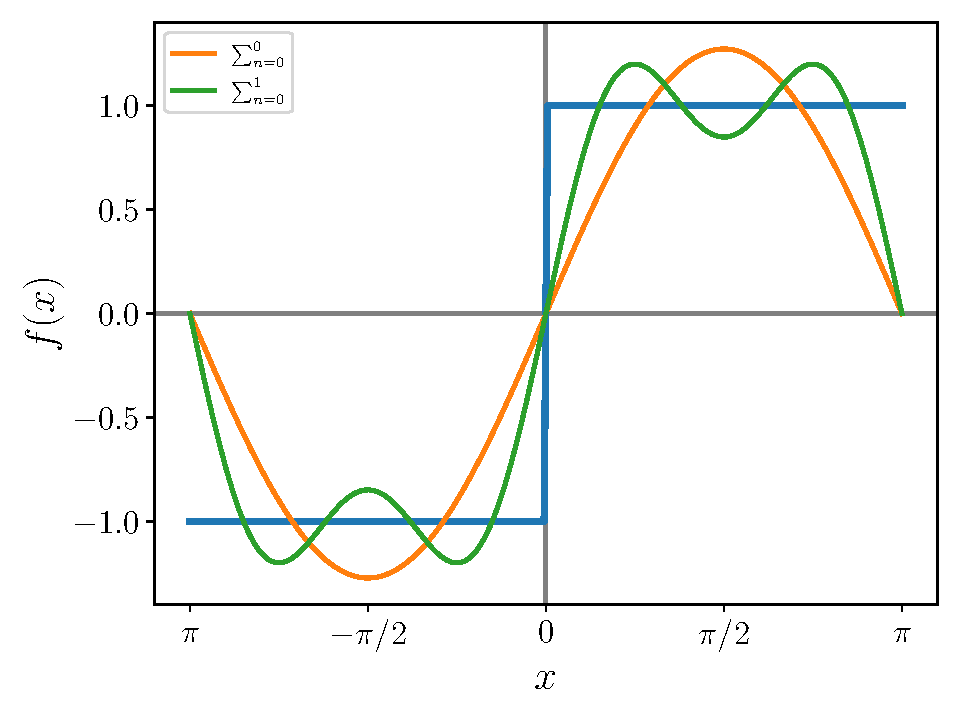
\includegraphics[scale=0.45]{figs/step-01.pdf}
\end{center} \pause

\cx
Agregando más términos:
\begin{center}
\only<2>  { 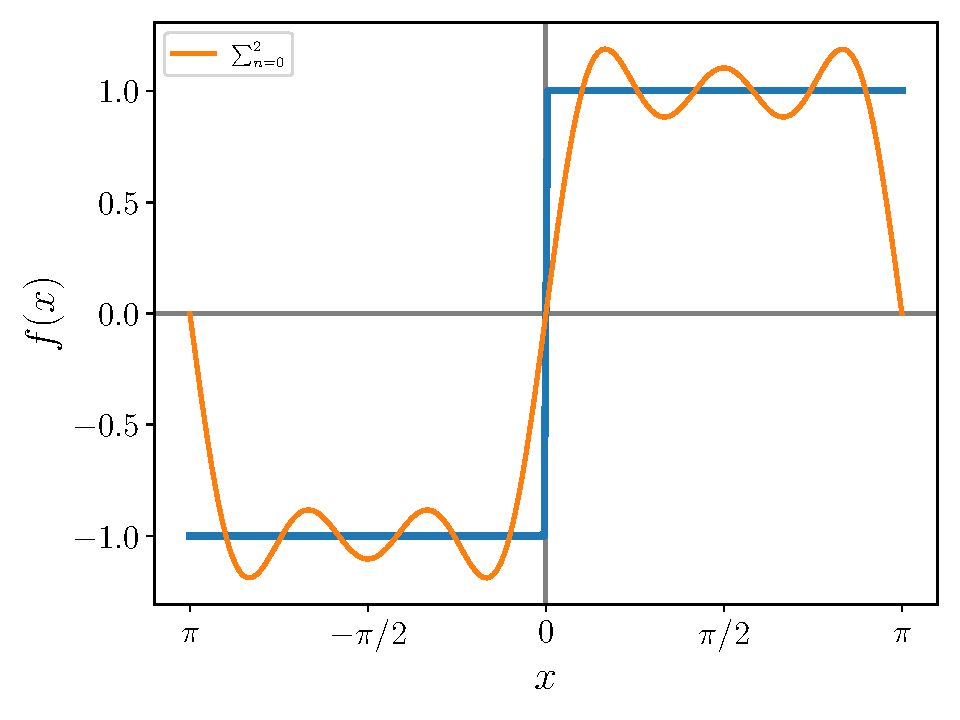
\includegraphics[scale=0.45]{figs/step-2.pdf} }
\only<3>  { 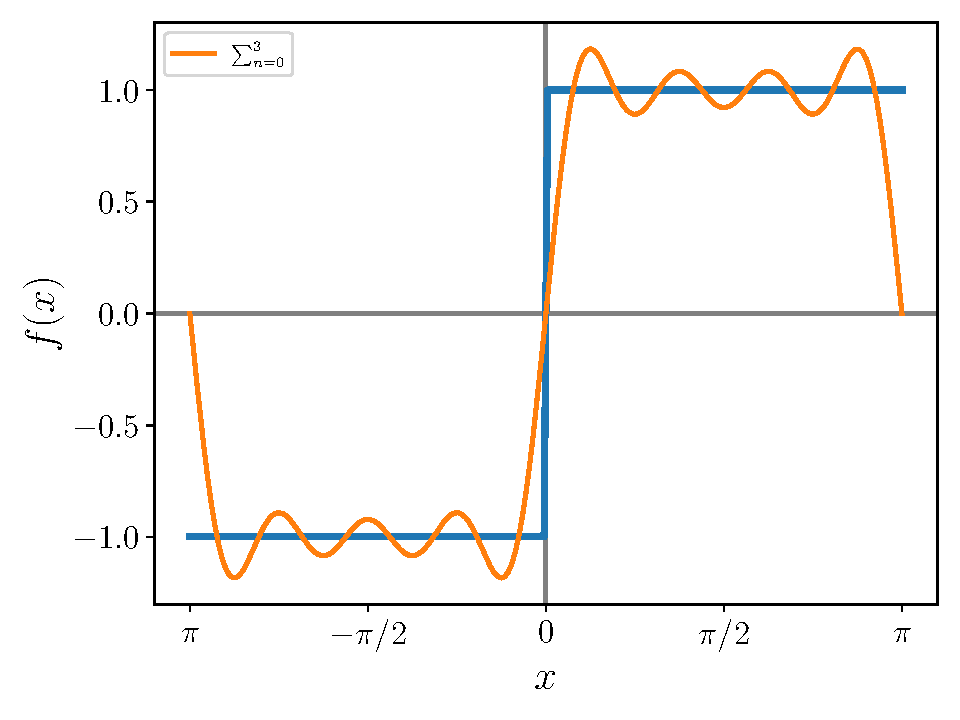
\includegraphics[scale=0.45]{figs/step-3.pdf} }
\only<4>  { 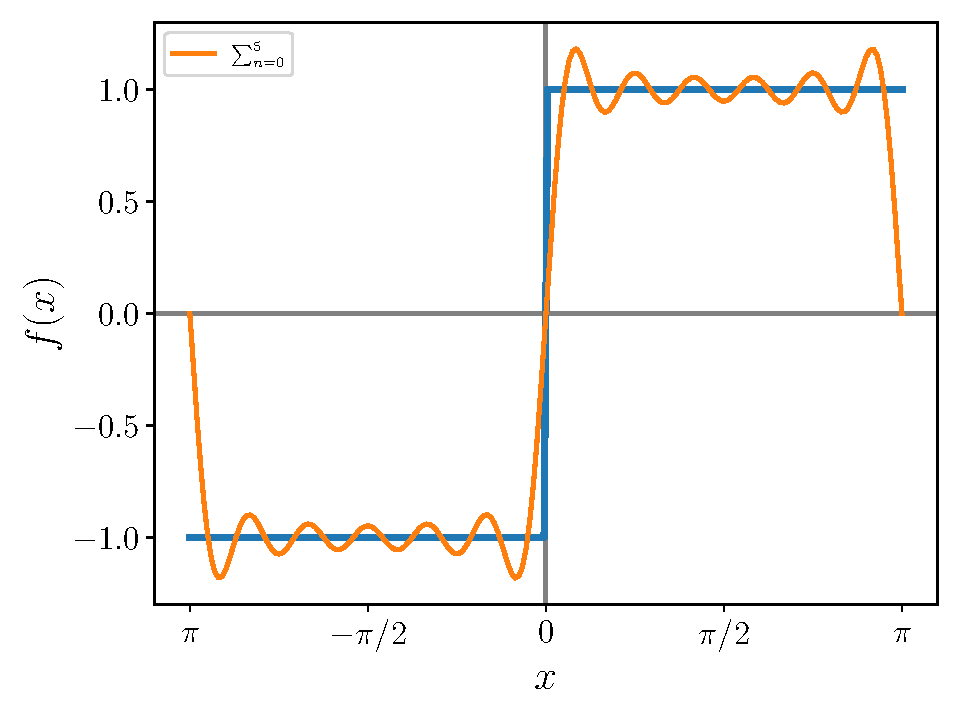
\includegraphics[scale=0.45]{figs/step-5.pdf} }
\end{center}

\only<2> {\[F_2(x) = \frac{4}{\pi} \left( \sen x + \frac{\sen 3x}{3} + \frac{\sen 5 x}{5} \right) \]}
\only<3> {\[F_3(x) = \frac{4}{\pi} \left( \sen x + \frac{\sen 3x}{3} + \frac{\sen 5 x}{5}  + \frac{\sen 7 x}{7}\right) \]}
\only<4> {\[F_5(x) = \frac{4}{\pi} \left( \cdots + \frac{\sen 9x}{9} + \frac{\sen 11 x}{11}  + \frac{\sen 13 x}{13}\right) \]}
\end{columns}
\end{frame}

\begin{frame}
\begin{columns}[t]
\cx
\textbf{Otro ejemplo:}
\begin{align*}
f(x) &= |x|, \quad -\pi < x < \pi \\
F(x) &= \frac{\pi}{2} - \frac{4}{\pi} \sum_{n \text{ impar}}^{\infty} \frac{\cos nx}{n^2}
\end{align*}

\begin{center}
    \only<1> {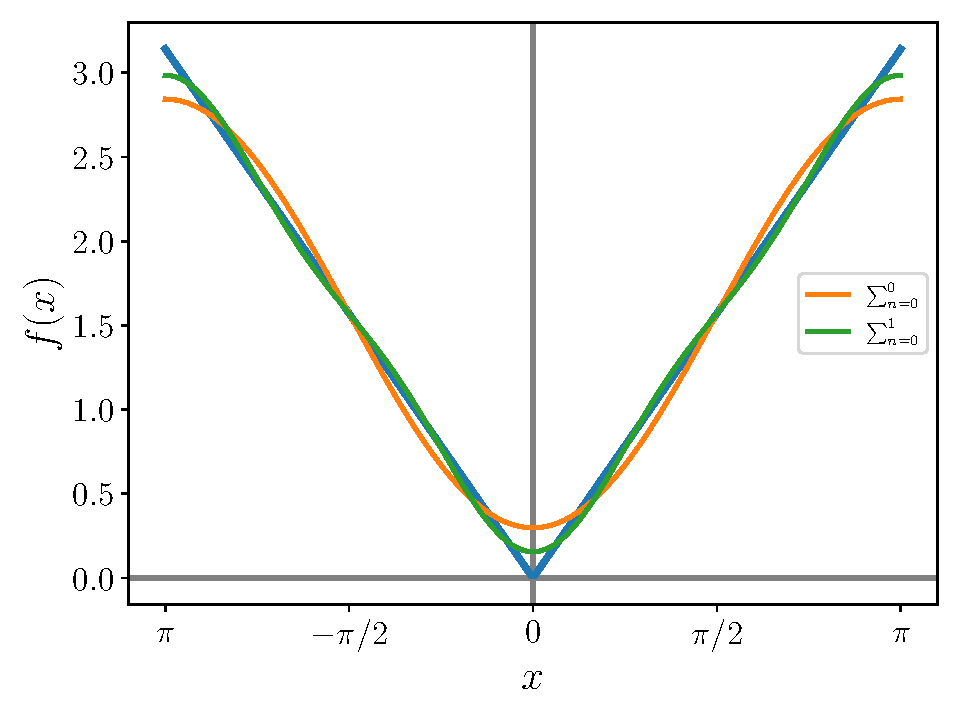
\includegraphics[scale=0.45]{figs/abs-01.pdf}}
    \only<2-> {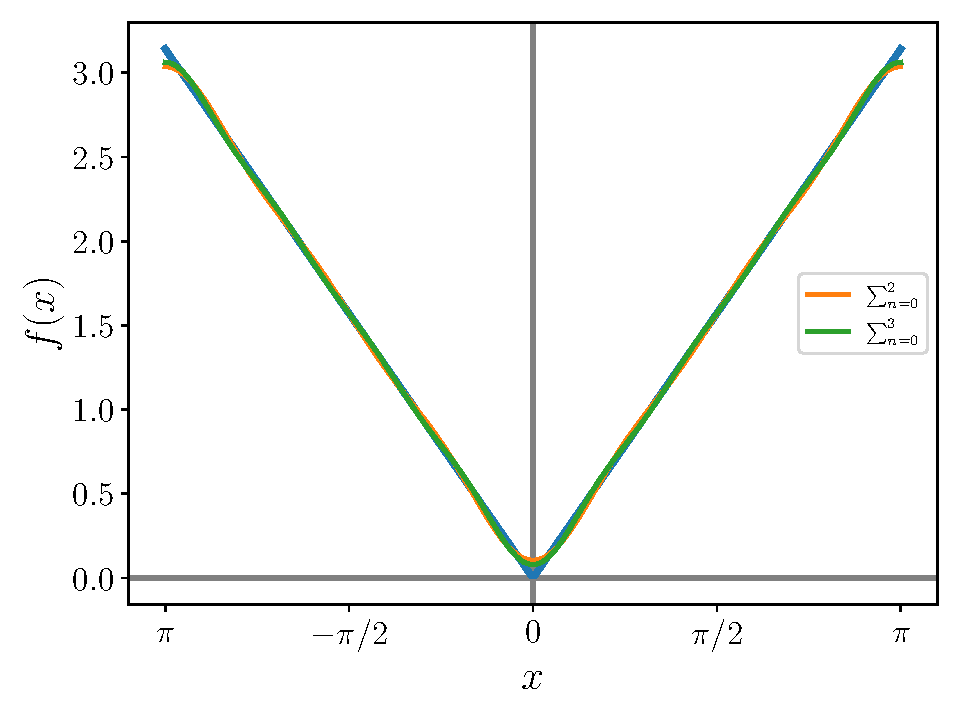
\includegraphics[scale=0.45]{figs/abs-23.pdf}}
\end{center}
\pause 

\cx
\textbf{Comparación con serie de potencias:}
\begin{multline*}
e^x = \sum_{n = 0}^{\infty} \frac{x^n}{n!} \\
= 1 + x + \frac{x^2}{2} + \frac{x^3}{6} + \frac{x^4}{24} + \frac{x^5}{120} + \cdots
\end{multline*}
\begin{center}
    \only<3> {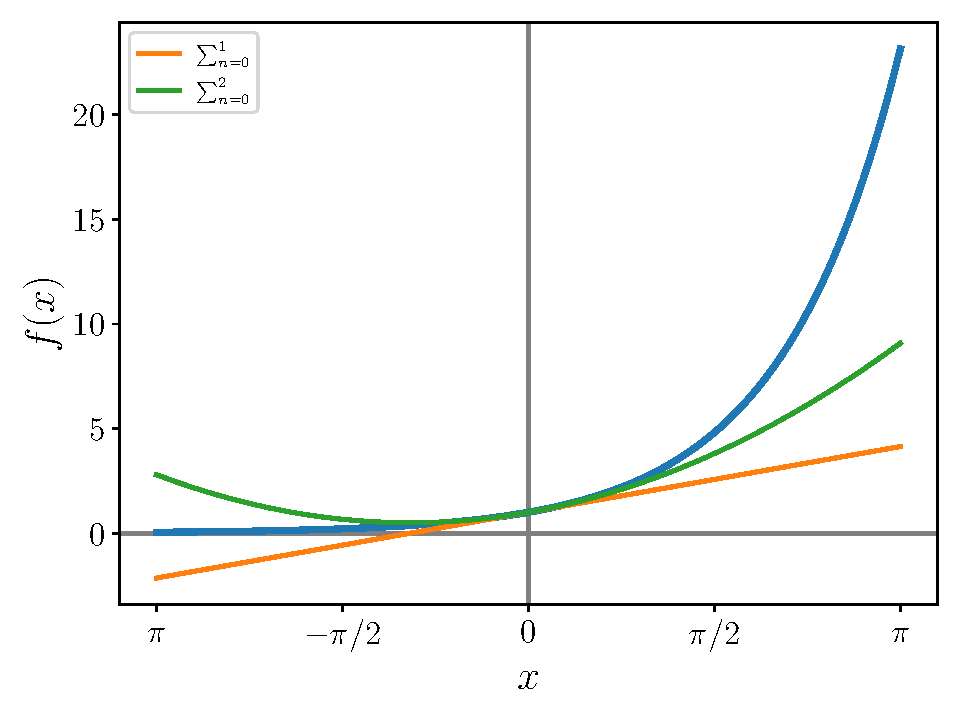
\includegraphics[scale=0.45]{figs/pot-12.pdf}}
    \only<4> {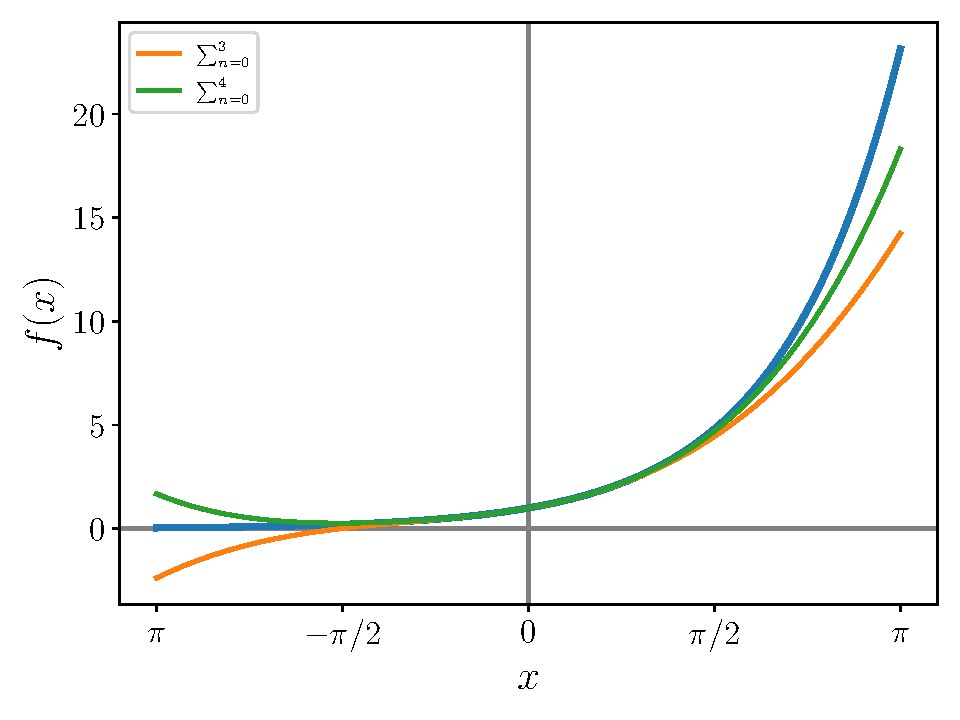
\includegraphics[scale=0.45]{figs/pot-34.pdf}}
\end{center}
\end{columns}
\end{frame}

\begin{frame}{Integral de Fourier}
\begin{columns}[t]
    \cw{0.3}
Del ejercicio 6 (Práctica 2):
\begin{equation*}
f_L(x) =
\begin{cases}
    0,& \quad -L < x < -1 \\
    1,& \quad -1 < x < 1 \\
    0,& \quad \phantom{-}1 < x < L \\
\end{cases}
\end{equation*}
\pause

\cw{0.6}
Función par:
\[ f(x) = a_0 + \sum_{n = 1}^{\infty} a_n \cos \frac{n \pi x}{L}, \quad a_0 = \frac{1}{2L} \int_{-1}^{1} dx = \frac{1}{L} \]
\[ a_n = \frac{1}{L} \int_{-1}^{1} \cos\frac{n \pi x}{L} \, dx = \frac{2}{L} \int_{0}^{1} \cos\frac{n \pi x}{L} \, dx = \frac{2}{L} \frac{\sen(n \pi / L)}{n \pi / L} \]
\end{columns}
\pause

\vspace{-1em}
\begin{columns}[c]
\cw{0.6}
\begin{center}
    \only<3> { 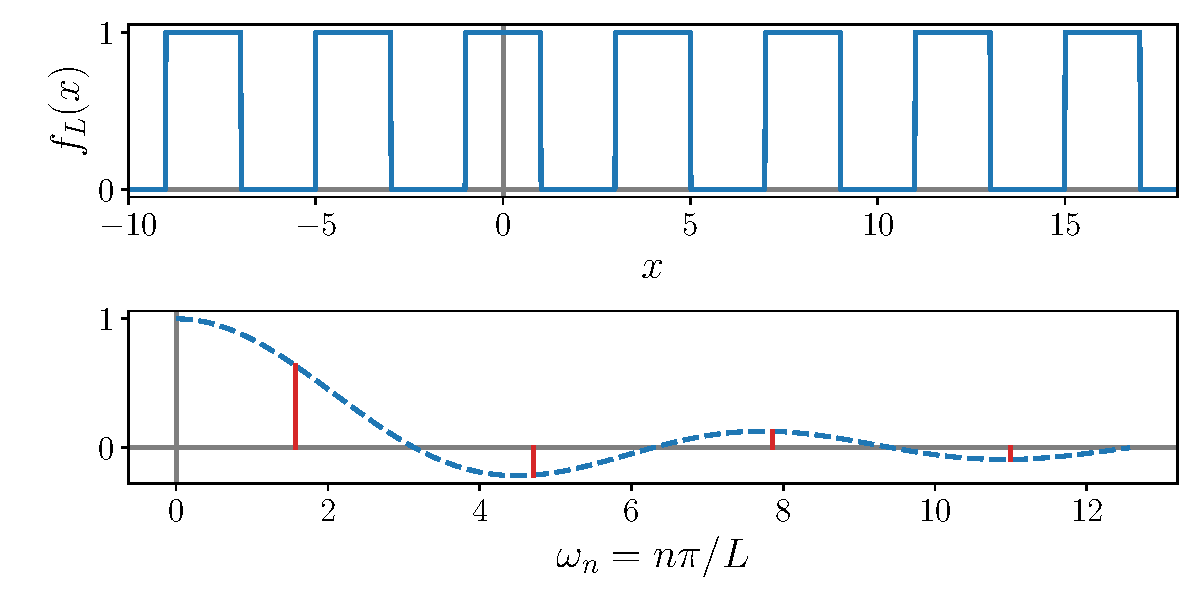
\includegraphics[scale=0.5]{figs/fig-01-1.pdf} }
    \only<4> { 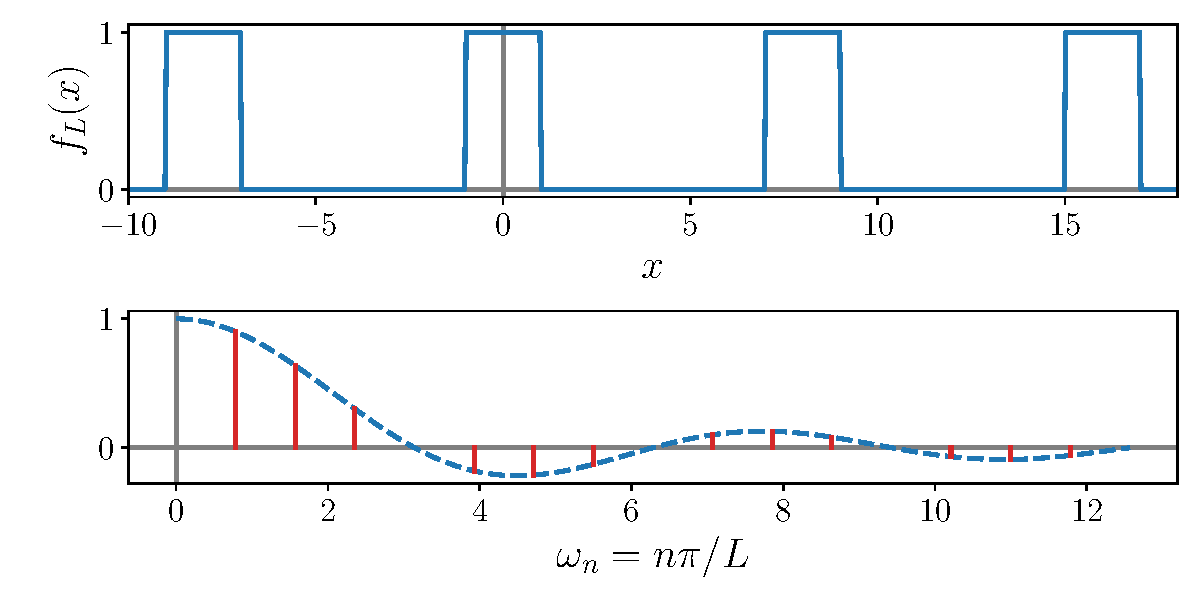
\includegraphics[scale=0.5]{figs/fig-01-2.pdf} }
    \only<5> { 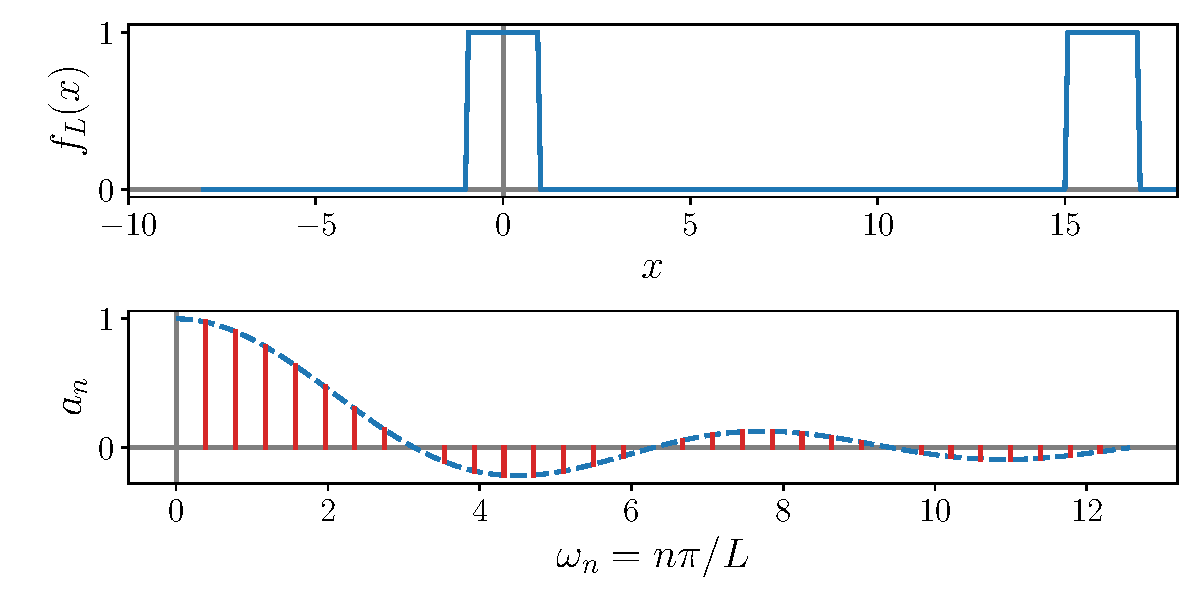
\includegraphics[scale=0.5]{figs/fig-01-3.pdf} }
\end{center}
\cw{0.4}
\only<3>{ \[ 2L = 4 \] } 
\only<4>{ \[ 2L = 8 \] } 
\only<5>{ \[ 2L = 16 \] } 
\end{columns}
\end{frame}

\begin{frame}
\begin{columns}[t]
\cx
Sea $f_L(x)$ una función de período $2L$:
\[ f_L(x) = a_0 + \sum_{i = 1}^{\infty} \left( a_n \cos \omega_n x + b_n \sen \omega_n x \right) \]
donde
\begin{align*}
    \omega_n &= \frac{n \pi}{L} \quad a_0= \frac{1}{2L} \int_{-L}^{L} f_L(x) \, dx \\
    a_n &= \frac{1}{L} \int_{-L}^{L} f_L(x) \cos \omega_n \, dx \\
    b_0 &= \frac{1}{L} \int_{-L}^{L} f_L(x) \sen \omega_n \, dx \\
\end{align*} \vspace{-3em}
\begin{multline*}
    f_L(x) = \frac{1}{2L} \int_{-L}^{L} f_L(\xi) \, d\xi \\
    + \frac{1}{L}\sum_{n = 1}^{\infty} \left[ \cos \omega_n x \int_{-L}^L f_L(\xi) \cos \omega_n \xi \, d\xi \right. \\
    + \left. \sen \omega_n x \int_{-L}^L f_L(\xi) \sen \omega_n \xi \, d\xi \right]
\end{multline*}
\pause

\cx
Ahora hacemos:
\[ \Delta \omega = \omega_{n+1} - \omega_n = \frac{(n + 1) \pi}{L} - \frac{n \pi}{L} = \frac{\pi}{L} \]
\begin{multline*}
    f_L(x) = \frac{1}{2L} \int_{-L}^{L} f_L(\xi) \, d\xi \\
    + \frac{1}{\pi}\sum_{n = 1}^{\infty} \left[ (\cos \omega_n x) \Delta \omega \int_{-L}^L f_L(\xi) \cos \omega_n \xi \, d\xi \right. \\
    + \left. (\sen \omega_n x) \Delta \omega \int_{-L}^L f_L(\xi) \sen \omega_n \xi \, d\xi \right]
\end{multline*}
\pause

Tomamos $L \rightarrow \infty$, y asumimos que
\[f(x) = \lim_{L \rightarrow \infty} f_L(x) \]
es \alert{absolutamente} integrable en el eje $x$:
\[ \lim_{a \rightarrow -\infty} \int_a^0 |f(x)| \, dx +  \lim_{b \rightarrow \infty} \int_0^b |f(x)| \, dx \mapsto \text{ existe} \]
\end{columns}
\end{frame}

\begin{frame}
\begin{columns}[t]
\cx
La representación de $f(x)$ por una \textbf{integral de Fourier}:
\begin{equation}
f(x) = \int_0^{\infty} \left[ A(\omega) \cos \omega x + B(\omega) \sen \omega x \right] \, d\omega 
\label{eq:01}
\end{equation}
donde:
\begin{equation}
    \begin{split}
    A(\omega) &= \frac{1}{\pi} \int_{-\infty}^{\infty} f(\xi) \cos \omega \xi \, d\xi \\
    B(\omega) &= \frac{1}{\pi} \int_{-\infty}^{\infty} f(\xi) \sen \omega \xi \, d\xi \\
    \end{split}
    \label{eq:02}
\end{equation}
\cx
\begin{theorem}[Integral de Fourier]
    Si $f(x)$ es suave a tramos en cada intervalo finito y tiene derivadas por derecha y por izquierda en cada punto, y si es absolutamente integrable en $(-\infty, \infty)$, entonces $f(x)$ puede representarse como una integral de Fourier \eqref{eq:01} con $A$ y $B$ dados por \eqref{eq:02}. En los puntos en que $f(x)$ es discontinua, el valor de la integral de Fourier es el promedio de los valores laterales de $f(x)$ en esos puntos.
\end{theorem}
\end{columns}
\end{frame}

\begin{frame}{Ejemplo}
\begin{columns}[c]
\cx
\[ f(x) =
    \begin{cases}
    1, \text{ si } |x| < 1 \\
    0, \text{ si } |x| > 1 
    \end{cases} 
\]

\begin{align*}
    A(\omega) &= \frac{1}{\pi} \int_{-\infty}^{\infty} f(\xi) \cos \omega \xi \, d\xi \\
              &= \frac{1}{\pi} \int_{-1}^{1} f(\xi) \cos \omega \xi \, d\xi = \left. \frac{\sen \omega \xi}{\pi \omega} \right|_{-1}^1 = \frac{2 \sen \omega}{\pi \omega} \\
    B(\omega) &= \frac{1}{\pi} \int_{-\infty}^{\infty} f(\xi) \sen \omega \xi \, d\xi = 0 
\end{align*}
\[    \boxed{ f(x) = \frac{2}{\pi} \int_0^{\infty} \frac{\cos \omega x \sen \omega}{w} \, d\omega } \]
\cx
\begin{center}
    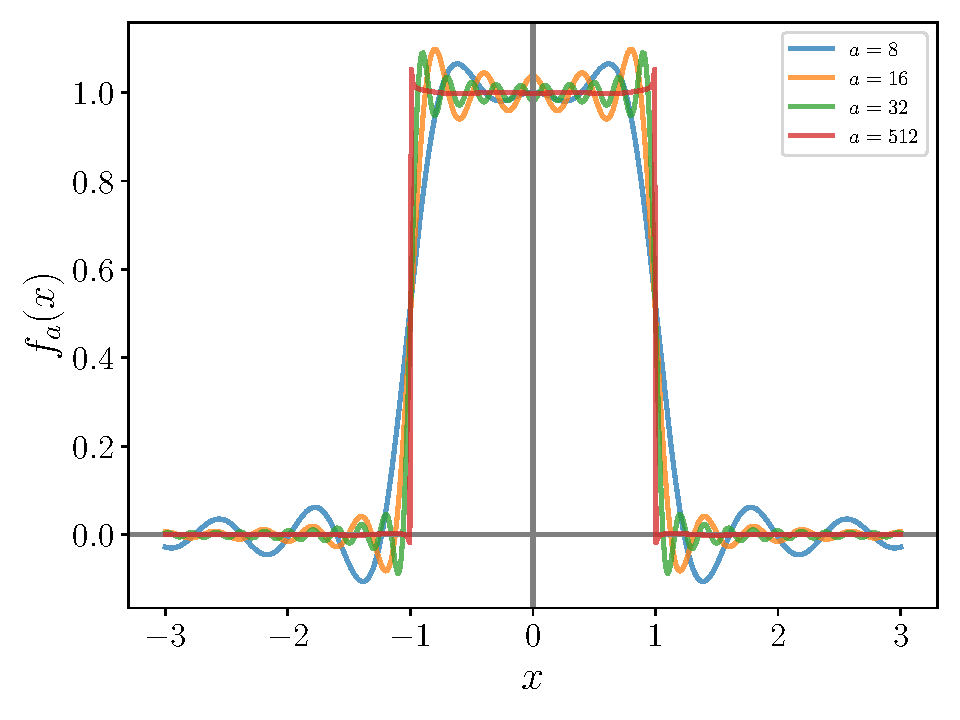
\includegraphics[scale=0.45]{figs/fig-02.pdf}
\end{center}
\end{columns}
\end{frame}

\begin{frame}{Transformaciones seno y coseno de Fourier}
\begin{columns}[t]
\cx
\textbf{Transformada coseno:}
Si $f(x)$ es par, de \eqref{eq:02}:
\begin{multline*}
    f(x) = \int_0^{\infty} A(\omega) \cos \omega x \, d\omega \\
 \text{con }    A(\omega) = \frac{2}{\pi} \int_0^{\infty} f(\xi) \cos \omega \xi d\xi
\end{multline*}
Llamamos $A(\omega) = \sqrt{ 2/\pi } \hat{f}_c(\omega)$:
\begin{subequations} \label{eq:tcf}
    \begin{equation}
    \hat{f}_c(\omega) = \sqrt{\frac{2}{\pi}} \int_0^{\infty} f(x) \cos \omega x \, dx \tag{\ref{eq:tcf}.a}
\end{equation}
    \begin{equation} 
    f(x) = \sqrt{\frac{2}{\pi}} \int_0^{\infty} \hat{f}_c(\omega) \cos \omega x \, d\omega \tag{\ref{eq:tcf}.b} 
    \end{equation}
\end{subequations}
\cx
\textbf{Transformada seno:}
Si $f(x)$ es impar, de \eqref{eq:02}:
\begin{multline*}
    f(x) = \int_0^{\infty} A(\omega) \sen \omega x \, d\omega \\
 \text{con }    B(\omega) = \frac{2}{\pi} \int_0^{\infty} f(\xi) \sen \omega \xi d\xi
\end{multline*}
Llamamos $B(\omega) = \sqrt{ 2/\pi } \hat{f}_s(\omega)$:
\begin{subequations} \label{eq:tsf}
    \begin{equation}
    \hat{f}_s(\omega) = \sqrt{\frac{2}{\pi}} \int_0^{\infty} f(x) \sen \omega x \, dx \tag{\ref{eq:tsf}.a}
\end{equation}
    \begin{equation} 
    f(x) = \sqrt{\frac{2}{\pi}} \int_0^{\infty} \hat{f}_c(\omega) \sen \omega x \, d\omega \tag{\ref{eq:tsf}.b} 
    \end{equation}
\end{subequations}
\end{columns}
\end{frame}

\begin{frame}{Transformada de Fourier}
\begin{columns}[t]
\cx
De las ecuaciones \eqref{eq:01} y \eqref{eq:02}:
\begin{multline*}
    f(x) = \frac{1}{\pi} \int_0^{\infty} \int_{-\infty}^{\infty} f(\xi) \left[ \cos \omega \xi \cos \omega x \right. \\
    \left. + \sen \omega \xi \sen \omega x \right] \, d\xi \, d\omega \\
    = \frac{1}{\pi} \int_0^{\infty} \left[ \int_{-\infty}^{\infty} f(\xi) \cos(\omega x - \omega \xi) d\xi \right] d\omega
\end{multline*}
$[\cdot]$ es una función par:
\begin{equation}\label{eq:03}
    f(x) = \frac{1}{2\pi} \int_{-\infty}^{\infty} \left[ \int_{-\infty}^{\infty} f(\xi) \cos(\omega x - \omega \xi) d\xi \right] d\omega
\end{equation}
Si usamos $\sen$ en vez de $\cos$, $[\cdot]$ es impar y
\begin{equation}\label{eq:04}
    \frac{1}{2\pi} \int_{-\infty}^{\infty} \left[ \int_{-\infty}^{\infty} f(\xi) \sen(\omega x - \omega \xi) d\xi \right] d\omega = 0
\end{equation}
\pause

\cx
Tomamos el integrando de \eqref{eq:03} y le sumamos $i$ multiplicado por el integrando de \eqref{eq:04}, usando la fórmula de Euler 
\[ e^{ix} = \cos x + i \sen x \]
obtenemos la \textbf{integral de Fourier compleja}:

\begin{equation*}
    f(x) = \frac{1}{2\pi} \int_{-\infty}^{\infty} \int_{-\infty}^{\infty} f(\xi) e^{i \omega(x - \xi)}  d\xi \, d\omega 
\end{equation*}

Escribiendo la exponencial de la suma como producto de exponenciales:

\begin{equation}\label{eq:ifc}
    f(x) = \frac{1}{\sqrt{2\pi}} \int_{-\infty}^{\infty} \left[ \int_{-\infty}^{\infty} \frac{1}{\sqrt{2\pi}} f(\xi) e^{-i \omega \xi}  d\xi \right] e^{i \omega x} \, d\omega 
\end{equation}
\end{columns}
\end{frame}

\begin{frame}{Transformada de Fourier}
\begin{columns}[c]
\cw{0.4}
\textbf{Transformada de Fourier} de $f$:
\begin{equation}\label{eq:TF}
    \hat{f}(\omega) = \frac{1}{\sqrt{2 \pi}} \int_{-\infty}^{\infty} f(x) e^{-i \omega x} \, dx
\end{equation}

\textbf{Transformada inversa de Fourier} de $\hat{f}$:
\begin{equation}\label{eq:TIF}
f(x) = \frac{1}{\sqrt{2 \pi}} \int_{-\infty}^{\infty} \hat{f}(\omega) e^{i \omega x} \, d\omega
\end{equation}

Otra nomenclatura:
\[ \hat{f} = \mathscr{F}(f), \qquad f = \mathscr{F}^{-1}(\hat{f}) \]

\cw{0.45}
\begin{theorem}[ Existencia de $\hat{f}$ ]
    Si $f(x)$ es absolutamente convergente en $(-\infty, \infty)$ y continua a tramos en intervalos finitos, entonces existe la transformada de Fourier $\hat{f}(\omega)$ de $f(x)$ dada por la ecuación \eqref{eq:TF}.
\end{theorem}
\end{columns}
\end{frame}

\begin{frame}{Ejemplos}
\begin{columns}[t]
\cx
Encontrar $\hat{f}$ de $f(x) = 1$ si $|x| < 1$ y $f(x) = 0$ en otro caso.
\begin{multline*}
    \hat{f}(\omega) = \frac{1}{\sqrt{2 \pi}} \int_{-1}^{1} e^{-i \omega x} \, dx \\
    = \frac{1}{\sqrt{2 \pi}} \left. \frac{e^{-i \omega x}}{-i \omega} \right|_{-1}^{1} = \frac{1}{-i \omega \sqrt{2 \pi} } \left( e^{-i \omega} - e^{i \omega} \right)
\end{multline*}
Usando la fórmula de Euler:
\[ e^{i \omega}- e^{-i \omega} = 2 i \sen \omega \]
resulta
\[ \hat{f}(\omega) = \sqrt{\frac{\pi}{2}} \frac{\sen \omega}{\omega} = \sqrt{\frac{\pi}{2}} \senc{\omega} \]
\pause

\cx
Encontrar $\hat{f}$ de $f(x) = e^{-a x}$ si $x > 0$ y $f(x) = 0$ si $x < 0$.

\begin{multline*}
    \hat{f}(\omega) = \frac{1}{\sqrt{2 \pi}} \int_{0}^{\infty} e^{-a x} e^{-i \omega x} \, dx \\
    = \frac{1}{\sqrt{2 \pi}} \left. \frac{e^{-(a + i \omega) x}}{-(a + i \omega)} \right|_{0}^{\infty}  \\ 
        = \frac{1}{\sqrt{2 \pi} (a + i \omega) } 
\end{multline*}
\end{columns}
\end{frame}

\begin{frame}{Interpretación física: espectro de energía}
\begin{columns}[t]
\cx
Representación \textbf{espectral}:
\[ f(x) = \frac{1}{\sqrt{2 \pi}} \int_{-\infty}^{\infty} \hat{f}(\omega) e^{i \omega x} \, d\omega \]
Densidad espectral $\hat{f}(\omega) \mapsto$ intensidad de $f(x)$ en $(\omega, \omega + d\omega)$.

\[ m x'' + k x = 0 \]
$\times x': \; m x' x'' + k x' x = 0$. Integrando:
\[ \dfrac{1}{2} m v^2 + \dfrac{1}{2} k x^2 = E_0 = \text{constante} \]
Solución general:
\[ x = a_1 \cos \omega_0 t + b_1 \sen \omega_0 t = \underbrace{c_1 e^{i \omega_0 t}}_{A} + \underbrace{c_{-1} e^{-i \omega_0 t}}_{B}\]
donde $\omega_0^2 = k/m$, $c_1 = (a_1 - i b_1)/2$, $c_{-1} = \bar{c}_1 = (a_1 + i b_1)/2$.
\pause

\cx
$x = A + B$, $x' = v = A' + B' = i \omega_0 (A - B)$:
\[ E_0 = \dfrac{1}{2} m (i \omega_0)^2 (A - B)^2 + \dfrac{1}{2} k (A + B)^2 \]
\begin{multline*}
    E_0 = \dfrac{1}{2}k \left[ -(A - B)^2 + (A + B)^2 \right] \\
    = 2 k A B = 2 k c_1 e^{i \omega_0 t} c_{-1} e^{-i \omega_0 t} \\
    = 2 k c_1 c_{-1} = 2 k |c_1|^2
\end{multline*}

Sistema más complejo: $x = f(t) \mapsto$ periódica: \\
\textbf{Espectro discreto:} $|c_1|^2 \mapsto |c_n|^2$ (conjunto contable de frecuencias aisladas).

Sistema más complejo: $x = f(t) \mapsto$ no periódica:
\[ \int_{-\infty}^{\infty} \left| \hat{f}(\omega) \right|^2 \, d\omega \]
es la \textbf{energía total} del sistema.
\end{columns}
\end{frame}

\begin{frame}{Algunas propiedades}
\begin{columns}[c]
\cx
\begin{theorem}[ Linealidad de $\mathscr{F}$ ]
    La transformada de Fourier es una \textbf{operación lineal}, esto es, para cualquier par de funciones $f(x)$ y $g(x)$ cuyas transformadas existan, y para cualesquiera constantes $a$ y $b$, la transformada de Fourier de $af + bg$ existe y
\begin{equation*}
    \mathscr{F}(a f + b g) = a \mathscr{F}(f) +  b \mathscr{F}(g)
\end{equation*}
\end{theorem} \pause

\begin{theorem}[Transformada de la derivada]
Sea $f(x)$ continua en $(-\infty, \infty)$ y $f(x) \rightarrow 0$ cuando $|x| \rightarrow \infty$. Entonces, si $f'(x)$ es absolutamente integrable en el eje $x$:
\[ \mathscr{F}[ f'(x)] = i \omega \mathscr{F}[f(x)]  \]
\end{theorem}
\pause 

\cx
La \textbf{convolución} $f * g$ de las funciones $f$ y $g$ se define complejo:
\begin{multline*}
    h(x) = (f * g)(x) = \int_{-\infty}^{\infty} f(\tau) g(x - \tau) \, d\tau \\
= \int_{-\infty}^{\infty} f(x - \tau) g(\tau) \, d\tau 
\end{multline*}
\pause 

\begin{theorem}[Convolución]
Sean $f(x)$ y $g(x)$ funciones acotadas, continuas por tramos, y absolutamente integrables en $(-\infty, \infty)$, entonces
\[ \mathscr{F}(f * g) = \sqrt{2 \pi} \mathscr{F}(f) \mathscr{F}(g) \]
\end{theorem}

\end{columns}
\end{frame}


\section*{Bibliografía}
\begin{frame}{Lecturas recomendadas}
\begin{itemize}
 \item \fullcite{kreyszig2011}. Capítulo 11 (11.7 -- 11.9).
 \item \fullcite{oneil2012es}. Capítulo 3.
 \item \fullcite{stroud2020}. Capítulos 9.
 \item \fullcite{kreyszig2011}. Capítulo 11 (11.1 -- 11.6).
 \item \fullcite{oneil2012es}. Capítulo 2.
 \item \fullcite{stroud2020}. Capítulos 7 y 8.
\end{itemize}
\end{frame}


\end{document}

